
%(BEGIN_QUESTION)
% Copyright 2010, Tony R. Kuphaldt, released under the Creative Commons Attribution License (v 1.0)
% This means you may do almost anything with this work of mine, so long as you give me proper credit

This fluid diagram shows the components and connections of a Bettis self-contained hydraulic module used to automatically shut off a ``line valve'' on a natural gas pipeline in the event of the pipeline pressure going outside of its limits (either falling below the low-pressure limit or rising above the high-pressure limit):

$$\includegraphics[width=15.5cm]{i04357x01.eps}$$

Identify all spool valve positions, and also trace the direction of oil flow, following a solenoid ``trip'' event.

\underbar{file i04357}
%(END_QUESTION)





%(BEGIN_ANSWER)

$$\includegraphics[width=15.5cm]{i04357x02.eps}$$

%(END_ANSWER)





%(BEGIN_NOTES)

\vskip 20pt \vbox{\hrule \hbox{\strut \vrule{} {\bf Virtual Trip-testing} \vrule} \hrule}

This question is a good candidate for a ``Virtual Trip-testing'' exercise.  Presenting the diagram to students, you pose an assignment whereby students must figure out how to test some component of this system to check that it will operate as intended to shut down the system in an abnormal (trip) condition, with some realistic limitation (e.g. power cannot be shut off to the load).  Students then propose various methods for executing the test.  Your job is to determine whether or not their proposed tests will achieve the desired result(s).

During and after the exercise, it is good to ask students follow-up questions such as:

\begin{itemize}
\item{} Where might our planned test strategy go wrong?  In other words, what thing(s) might happen to foil our test, either to invalidate the results or to not honor the stated limitation(s)?
\item{} Suppose the limitation were different.  How would this affect our ability to carry out the test?
\item{} Is the last test strategy best one we could execute?
\end{itemize}



%INDEX% Final Control Elements, valve: fail-safe solenoids
%INDEX% Process: pipeline safety shutoff valve

%(END_NOTES)


